\section{Data Analysis}
For the two areas of interest, Glostrup and Herlev, TTS supplied data from detectors for a period of a couple of weeks in november 2007.

This period is generally accepted as the beginning of the winter season and as such the traffic is expected to be high and as such the data serves as a worst-case scenario.

The detector input data is used to establish traffic input levels according to the day and time of day. Also, since the data does not represent exactly what traffic each link observed during the period, it is analyzed to establish some estimates of the traffic for missing links.

The format of the data is:

\begin{table}[!ht]
\begin{center}
\begin{tabular}{c|c|c|c|c}
\textbf{Date} & \textbf{Time} & \textbf{D1} & \textbf{...} & \textbf{DN} \\ \hline
13-11-2007 & 08:42:56 & 39 & ... & 35 \\
13-11-2007 & 08:44:26 & 38 & ...  & 28 \\
\end{tabular}
\end{center}
\caption{Format of TTS supplied detector data}
\label{tab:dataformat}
\end{table}

Thus each detector, named D\textit{N}, has a column where the numbers are the detected vehicles since last detection. The detections are made once for every cycle thus there will be some variations in the time between measurements due to the adjustments to cycle time, which are made by DOGS.

It was agreed with DRD that the temporal resolution be fixed at 15 minutes. This accumulation was performed by indexing time within the data period into 15 minute bins and summing detections from the last 15 minutes.

Multiple data files - for different sets of detectors - was received for each area. Since the data period was not identical over the data files it was necessary to perform some cleanup in order to generate accumulated data in which all detectors were represented.

\begin{table}[!ht]
\begin{center}
\begin{tabular}{c|c|c|c}
\textbf{Area} & \textbf{From} & \textbf{To} & \textbf{Detectors} \\ \hline
Herlev & 13-11-2007 20:45 & 28-11-2007 09:45 & D3-D8, D13-D15, D18 \\
Glostrup & 13-11-2007 08:45 & 26-11-2007 14:15 & D1-D14 \\
\end{tabular}
\end{center}
\caption{Periods of aggregated and cleaned data sets}
\label{tab:dataperiod}
\end{table}

I have performed analyses for each area in order to reach the required estimates for input sizes and proportions in route choice in Vissim.

\subsection{Herlev}

The first graph I present, see Figure \ref{fig:herlev_props} shows how the overall traffic fluctuates between workdays and weekends. It also shows that there is slightly more northgoing traffic.

\begin{figure}[!ht]
\begin{center}
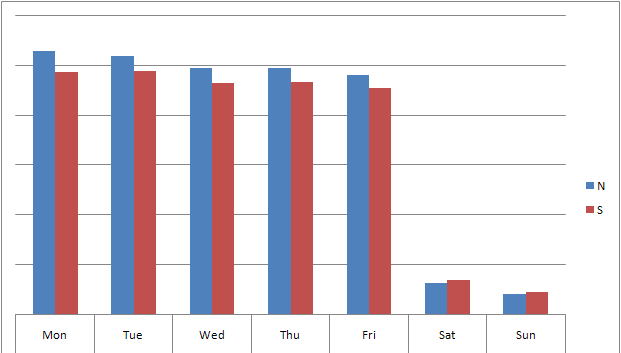
\includegraphics[scale=0.35]{herlev_direction_proportions.png} 
\end{center}
\caption{Daily- and directional variations in Herlev}
\label{fig:herlev_props}
\end{figure}

The next graph, see Figure \ref{fig:herlev_commuter}, shows the usual commuter- and lunch traffic patterns. The data from all mondays to fridays in the dataset have almost identical temporal distributions and thus the graph shows summarized data from workdays.

\begin{figure}[!ht]
\begin{center}
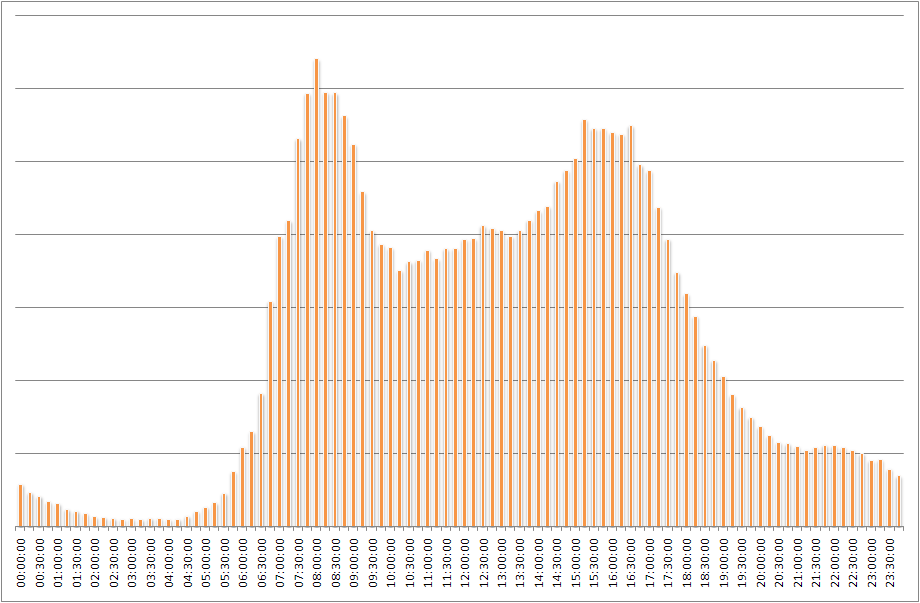
\includegraphics[scale=0.4]{herlev_workday_distribution.png} 
\end{center}
\caption{Distribution of traffic throughout workdays in Herlev}
\label{fig:herlev_commuter}
\end{figure}

By comparing the workday distribution to the detected traffic in the weekend, see Figure \ref{fig:herlev_weekends} - and at the same time looking and the proportions of demand in Figure \ref{fig:herlev_props} - it is clear that O3 in Herlev is heavily used by commuters. Traffic is almost identically distributed on saturdays and sundays and the graph shows summarized data for the weekend.

\begin{figure}[!ht]
\begin{center}
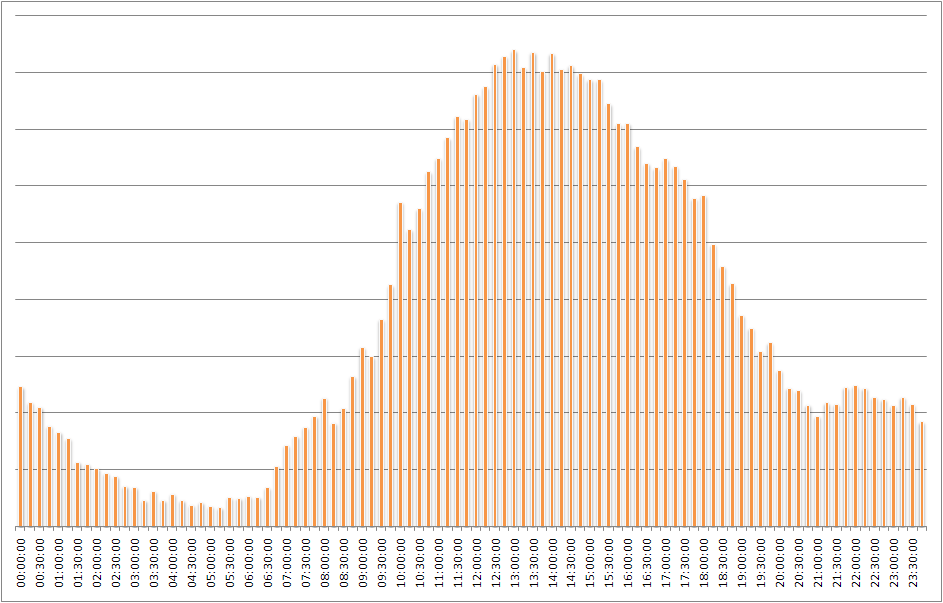
\includegraphics[scale=0.4]{herlev_weekend_distribution.png} 
\end{center}
\caption{Distribution of traffic throughout the weekend in Herlev}
\label{fig:herlev_weekends}
\end{figure}

As the directional proportions remain the same as in Figure \ref{fig:herlev_props}, the last two graphs summarize on direction.